\documentclass
[
  fontsize = 10pt,
  compress = true,
  ngerman,
  dvipsnames
]
{beamer}

\usepackage[utf8]{inputenc}
\usepackage[T1]{fontenc}
\usepackage{lmodern}
\usepackage{babel}
\usepackage{enumerate}
\usepackage{siunitx}
\usepackage{tikz}

\usetheme{Rochester}

% verdeckte Elemente grau anzeigen
\setbeamercovered{transparent}

% Komma als Trennzeichen
\sisetup{locale=DE, group-minimum-digits=4}

% fuer die geschweiften Klammern
\usetikzlibrary{decorations.pathreplacing}

% ------------------------------------------------------------------------------
\begin{document}
% ------------------------------------------------------------------------------

\newcommand{\sectiontitle}{}

\begin{frame}
  \frametitle{Geraden und Dreiecke in der Ebene}
  \begin{block}{Aufgabe 1}
    In welchem Punkt schneidet die Gerade $g_1$, die durch die Punkte $P$
    und $Q$ festgelegt ist, die Gerade $g_2$, die durch die Punkte $R$ und
    $S$ verfäuft?
  \end{block}
  \begin{block}{Aufgabe 2}
    Nimmt man die $x$-Achse als dritte Gerade hinzu, ergibt sich zusammen
    mit den Geraden $g_1$ und $g_2$ ein Dreieck.
    \begin{enumerate}[{2}.1]
      \item Bestimme den Umfang dieses Dreiecks.
      \item Bestimme den Flächeninhalt dieses Dreiecks.
      \item Bestimme die Innenwinkel dieses Dreiecks.
    \end{enumerate}
  \end{block}
\end{frame}

% ------------------------------------------------------------------
\renewcommand{\sectiontitle}{Aufgabe 1: Bestimmen des Schnittpunkts}
% ------------------------------------------------------------------

\newcommand{\PP}{P\left(\num{7}\;\middle|\;\num{6}\right)}
\newcommand{\PQ}{Q\left(\num{4}\;\middle|\;\num{15}\right)}
\newcommand{\PR}{R\left(\num{-5}\;\middle|\;\num{-16}\right)}
\newcommand{\PS}{S\left(\num{12}\;\middle|\;\num{18}\right)}

\begin{frame}
  \frametitle{\sectiontitle}
  \begin{block}{Beispiel}
    Gegeben seien folgende Punkte:
    \begin{equation*}
      \PP \quad \PQ \qquad \PR \quad \PS
    \end{equation*}
  \end{block}
  \bigskip

  Daraus müssen zunächst die Geradenparameter $m$ und $b$
  der beiden Geraden ermittelt werden:
  \begin{equation*}
    \begin{split}
      \text{aus $P$ und $Q$}\quad\rightsquigarrow\quad g_1:f(x)&=m_1\cdot x+b_1 \\[1ex]
      \text{aus $R$ und $S$}\quad\rightsquigarrow\quad g_2:f(x)&=m_2\cdot x+b_2
    \end{split}
  \end{equation*}
\end{frame}

\begin{frame}
  \frametitle{\sectiontitle}
  \framesubtitle{Schritt 1: Aufstellen der Geradengleichungen}
  Die Steigung $m$ lässt sich aus den Koordinaten zweier
  Punkte $P_1(x_1\mid y_1)$ und $P_2(x_2\mid y_2)$ berechnen,
  die auf der Geraden liegen:
  \begin{equation*}
    m=\frac{y_2-y_1}{x_2-x_1}
  \end{equation*}

  \pause

  Mit den Punkten $\PP$ und $\PQ$ erhält man:
  \begin{equation*}
    m_1=\frac{6-15}{7-4}=\frac{-9}{3}=-3
  \end{equation*}

  \alert{Wichtig ist hierbei, dass der Punkt mit der kleineren $x$-Koordinate den Index 1 erhält!}
\end{frame}

\begin{frame}
  \frametitle{\sectiontitle}
  \framesubtitle{Schritt 1: Aufstellen der Geradengleichungen}
  Sobald man die Steigung $m$ ermittelt hat, kann man mit einem der
  beiden bekannten Punkte den $y$-Achsenabschnitt $b$ bestimmen
  \bigskip

  \pause

  Verwendet man zum Beispiel Punkt $\PQ$, erhält man für $b$:
  \begin{alignat*}{3}
                   &\quad &  y&=m\cdot x+b  & \quad&\mid\text{$Q$ und $m$ einsetzen} \\
    \Rightarrow    &\quad & 15&=-3\cdot 4+b & \quad&        \\
    \Leftrightarrow&\quad & 15&=-12+b       & \quad&\mid+12 \\
    \Leftrightarrow&\quad & 27&=b           & \quad&
  \end{alignat*}

  \pause

  Damit ist die Funktionsgleichung der ersten Gerade ermittelt:
  \begin{equation*}
    g_1:f(x)=-3x+27
  \end{equation*}
\end{frame}

\begin{frame}
  \frametitle{\sectiontitle}
  \framesubtitle{Schritt 1: Aufstellen der Geradengleichungen}
  Aus den Punkten $\PR$ und $\PS$ ergibt sich die Steigung von $g_2$:
  \begin{equation*}
    m_2=\frac{y_2-y_1}{x_2-x_1}=\frac{18-(-16)}{12-(-5)}=\frac{34}{17}=2
  \end{equation*}
\end{frame}

\begin{frame}
  \frametitle{\sectiontitle}
  \framesubtitle{Schritt 1: Aufstellen der Geradengleichungen}
  Zur Bestimmung des $y$-Achsenabschnitts von $g_2$ eignet sich
  Punkt $\PS$ etwas besser, weil dessen Koordinaten keine
  negativen Vorzeichen besitzen.
  \begin{alignat*}{3}
                   &\quad &  y&=m\cdot x+b  & \quad&\mid\text{$S$ und $m$ einsetzen} \\
    \Rightarrow    &\quad & 18&=2\cdot 12+b & \quad&        \\
    \Leftrightarrow&\quad & 18&=24+b        & \quad&\mid-24 \\
    \Leftrightarrow&\quad & -6&=b           & \quad&
  \end{alignat*}

  \pause

  Damit ist die Funktionsgleichung der zweiten Gerade ermittelt:
  \begin{equation*}
    g_2:f(x)=2x-6
  \end{equation*}
\end{frame}

\begin{frame}
  \frametitle{\sectiontitle}
  \framesubtitle{Schritt 2: Lösen des linearen Gleichungssystems}
  Den Schnittpunkt beider Geraden erhält man nun als Lösung des
  Gleichungssystems:
  \begin{equation*}
    \left|
    \begin{aligned}
      f(x)=y&=-3x+27 \\
      f(x)=y&=2x-6
    \end{aligned}
    \right.
  \end{equation*}

  \pause

  Da beide Gleichungen bereits nach $y$ aufgelöst sind, bietet
  sich zur Lösung das \emph{Gleichsetzungsverfahren} an, also:
  \begin{equation*}
    -3x+27=2x-6
  \end{equation*}
\end{frame}

\begin{frame}
  \frametitle{\sectiontitle}
  \framesubtitle{Schritt 2: Lösen des linearen Gleichungssystems}
  Die $x$-Koordinate des Schnittpunkts erhält man durch das
  Auflösen der Gleichung nach $x$:
  \begin{alignat*}{3}
                   &\quad &      -3x+27&=2x-6 & \quad&\mid+3x  \\
    \Leftrightarrow&\quad &          27&=5x-6 & \quad&\mid+6   \\
    \Leftrightarrow&\quad &        33&=5x     & \quad&\mid\;:5 \\
    \Leftrightarrow&\quad & \num{6.6}&=x      & \quad&
  \end{alignat*}
\end{frame}

\begin{frame}
  \frametitle{\sectiontitle}
  \framesubtitle{Schritt 3: Berechnen des zugehörigen Funktionswertes}
  Die $y$-Koordinate des Schnittpunkts erhält man durch das
  Einsetzen der $x$-Koordinate in eine der beiden Geradengleichungen:
  \begin{equation*}
    \begin{split}
      f(x)&=2x-6 \\
      \Rightarrow\quad
      f(\num{6.6})&=2\cdot\num{6.6}-6=\num{7.2}
    \end{split}
  \end{equation*}
  
  \pause

  Der gesuchte Schnittpunkt ist also der Punkt $C(\num{6.6}\mid\num{7.2})$.
\end{frame}

\begin{frame}
  \frametitle{Geraden und Dreiecke in der Ebene}
  \begin{block}{Aufgabe 1}
    In welchem Punkt schneidet die Gerade $g_1$, die durch die Punkte $P$
    und $Q$ festgelegt ist, die Gerade $g_2$, die durch die Punkte $R$ und
    $S$ verfäuft?
  \end{block}
  \begin{block}{Aufgabe 2}
    Nimmt man die $x$-Achse als dritte Gerade hinzu, ergibt sich zusammen
    mit den Geraden $g_1$ und $g_2$ ein Dreieck.
    \begin{enumerate}[{2}.1]
      \item Bestimme den Umfang dieses Dreiecks.
      \item Bestimme den Flächeninhalt dieses Dreiecks.
      \item Bestimme die Innenwinkel dieses Dreiecks.
    \end{enumerate}
  \end{block}
\end{frame}

% --------------------------------------------------------------
\renewcommand{\sectiontitle}{Aufgabe 2.1: Bestimmen des Umfangs}
% --------------------------------------------------------------

\begin{frame}
  \frametitle{\sectiontitle}
  \begin{itemize}
    \item Zuerst werden die fehlenden Koordinaten der beiden Eckpunkte
          $A$ und $B$ des Dreiecks benötigt. Diese ergeben sich aus den
          \textbf{Nullstellen} der Geraden.
    \item Aus den Koordinatendifferenzen lassen sich dann die Längen der
          Dreiecksseiten mithilfe des Satzes von \textbf{Pythagoras}
          berechnen.
  \end{itemize}
\end{frame}

\begin{frame}
  \frametitle{\sectiontitle}
  \framesubtitle{Schritt 1: Berechnen der Nullstellen}
  \centering
  \begin{tikzpicture}[scale=0.7]
    \coordinate (A1) at (6.333,   8.000);
    \coordinate (A2) at (9.333,  -1.000);
    \coordinate (B1) at (2.500,  -1.000);
    \coordinate (B2) at (7.000,   8.000);
    % x-axis
    \draw[line width=0.6pt, ->, >=stealth] (-1.000, 0) -- (12.000, 0) node[below] {\small$x$};
    % x scale
    \draw[line width=0.6pt] ( 1, 0.1) -- ( 1, -0.1) node[below] {\small1};
    \draw[line width=0.6pt] ( 2, 0.1) -- ( 2, -0.1);
    \draw[line width=0.6pt] ( 3, 0.1) -- ( 3, -0.1);
    \draw[line width=0.6pt] ( 4, 0.1) -- ( 4, -0.1);
    \draw[line width=0.6pt] ( 5, 0.1) -- ( 5, -0.1) node[below] {\small5};
    \draw[line width=0.6pt] ( 6, 0.1) -- ( 6, -0.1);
    \draw[line width=0.6pt] ( 7, 0.1) -- ( 7, -0.1);
    \draw[line width=0.6pt] ( 8, 0.1) -- ( 8, -0.1);
    \draw[line width=0.6pt] ( 9, 0.1) -- ( 9, -0.1);
    \draw[line width=0.6pt] (10, 0.1) -- (10, -0.1) node[below] {\small10};
    \draw[line width=0.6pt] (11, 0.1) -- (11, -0.1);
    % y-axis
    \draw[line width=0.6pt, ->, >=stealth] (0, -1.000) -- (0, 8.000) node[left] {\small$y$};
    % y scale
    \draw[line width=0.6pt] (0.1, 1) -- (-0.1, 1) node[left] {\small1};
    \draw[line width=0.6pt] (0.1, 2) -- (-0.1, 2);
    \draw[line width=0.6pt] (0.1, 3) -- (-0.1, 3);
    \draw[line width=0.6pt] (0.1, 4) -- (-0.1, 4);
    \draw[line width=0.6pt] (0.1, 5) -- (-0.1, 5) node[left] {\small5};
    \draw[line width=0.6pt] (0.1, 6) -- (-0.1, 6);
    \draw[line width=0.6pt] (0.1, 7) -- (-0.1, 7);
    % lines
    \draw[line width=0.5pt] (A1) -- (A2);
    \draw[line width=0.5pt] (B1) -- (B2);
    % points
    \fill (3, 0) circle[radius=1.4pt] node[above left]{\small$A$};
    \fill (9, 0) circle[radius=1.4pt] node[above right]{\small$B$};
    \fill (6.6, 7.2) circle[radius=1.4pt] node[right]{\small$C(\num{6.6}\mid\num{7.2})$};
  \end{tikzpicture}
\end{frame}

\begin{frame}
  \frametitle{\sectiontitle}
  \framesubtitle{Schritt 1: Berechnen der Nullstellen}
  Die Nullstelle ist der Wert, den man für $x$ einsetzen muss,
  damit als Ergebnis 0 herauskommt:
  \begin{alignat*}{3}
                   &\quad & g_1:f(x)&=-3x+27 & \quad&\mid\text{setze $y=0$} \\
                   &\quad &        0&=-3x+27 & \quad&\mid-27                \\
    \Leftrightarrow&\quad &      -27&=-3x    & \quad&\mid\;:(-3)            \\
    \Leftrightarrow&\quad &        9&=x      & \quad&                       \\[2ex]
    \pause
                   &\quad & g_2:f(x)&=2x-6 & \quad&\mid\text{setze $y=0$}   \\
                   &\quad &        0&=2x-6 & \quad&\mid+6                   \\
    \Leftrightarrow&\quad &        6&=2x   & \quad&\mid\;:2                 \\
    \Leftrightarrow&\quad &        3&=x    & \quad&
  \end{alignat*}
\end{frame}

\begin{frame}
  \frametitle{\sectiontitle}
  \framesubtitle{Schritt 1: Berechnen der Nullstellen}
  Die beiden Nullstellen lauten also 9 und 3.
  Die kleinere von beiden wird als $x$-Koordinate dem Punkt $A$ zugeordnet
  und die größere von beiden dem Punkt $B$.
  \bigskip\par
  \centering
  \begin{tikzpicture}[scale=0.7]
    \coordinate (A1) at (6.333,   8.000);
    \coordinate (A2) at (9.333,  -1.000);
    \coordinate (B1) at (2.500,  -1.000);
    \coordinate (B2) at (7.000,   8.000);
    % clipping
    \clip (-1.5, -1.0) rectangle (12.5, 4.5);
    % x-axis
    \draw[line width=0.6pt, ->, >=stealth] (-1.000, 0) -- (12.000, 0) node[below] {\small$x$};
    % x scale
    \draw[line width=0.6pt] ( 1, 0.1) -- ( 1, -0.1) node[below] {\small1};
    \draw[line width=0.6pt] ( 2, 0.1) -- ( 2, -0.1);
    \draw[line width=0.6pt] ( 3, 0.1) -- ( 3, -0.1);
    \draw[line width=0.6pt] ( 4, 0.1) -- ( 4, -0.1);
    \draw[line width=0.6pt] ( 5, 0.1) -- ( 5, -0.1) node[below] {\small5};
    \draw[line width=0.6pt] ( 6, 0.1) -- ( 6, -0.1);
    \draw[line width=0.6pt] ( 7, 0.1) -- ( 7, -0.1);
    \draw[line width=0.6pt] ( 8, 0.1) -- ( 8, -0.1);
    \draw[line width=0.6pt] ( 9, 0.1) -- ( 9, -0.1);
    \draw[line width=0.6pt] (10, 0.1) -- (10, -0.1) node[below] {\small10};
    \draw[line width=0.6pt] (11, 0.1) -- (11, -0.1);
    % y-axis
    \draw[line width=0.6pt, ->, >=stealth] (0, -1.000) -- (0, 8.000) node[left] {\small$y$};
    % y scale
    \draw[line width=0.6pt] (0.1, 1) -- (-0.1, 1) node[left] {\small1};
    \draw[line width=0.6pt] (0.1, 2) -- (-0.1, 2);
    \draw[line width=0.6pt] (0.1, 3) -- (-0.1, 3);
    \draw[line width=0.6pt] (0.1, 4) -- (-0.1, 4);
    \draw[line width=0.6pt] (0.1, 5) -- (-0.1, 5) node[left] {\small5};
    \draw[line width=0.6pt] (0.1, 6) -- (-0.1, 6);
    \draw[line width=0.6pt] (0.1, 7) -- (-0.1, 7);
    % lines
    \draw[line width=0.5pt] (A1) -- (A2);
    \draw[line width=0.5pt] (B1) -- (B2);
    % points
    \fill (3, 0) circle[radius=1.4pt] node[above left]{\small$A(\num{3}\mid\num{0})$};
    \fill (9, 0) circle[radius=1.4pt] node[above right]{\small$B(\num{9}\mid\num{0})$};
    \fill (6.6, 7.2) circle[radius=1.4pt] node[right]{\small$C(\num{6.6}\mid\num{7.2})$};
  \end{tikzpicture}
\end{frame}

\begin{frame}
  \frametitle{\sectiontitle}
  \framesubtitle{Schritt 2: Berechnen der Seitenlängen}
  Die Länge der Seite $c$ ist nun einfach der Abstand zwischen den beiden
  Nullstellen:
  \begin{equation*}
    c=B_x-A_x=9-3=6
  \end{equation*}

  \pause

  Um die Längen der (schrägen) Seiten $a$ und $b$ zu bestimmen, kann
  man den Satz des Pythagoras verwenden. Sobald man die Höhe des Dreiecks
  als Hilfslinie einzeichnet, wird die Situation klar:
\end{frame}

\begin{frame}
  \frametitle{\sectiontitle}
  \framesubtitle{Schritt 2: Berechnen der Seitenlängen}
  \centering
  \begin{tikzpicture}[scale=0.7]
    \coordinate (A1) at (6.333,   8.000);
    \coordinate (A2) at (9.333,  -1.000);
    \coordinate (B1) at (2.500,  -1.000);
    \coordinate (B2) at (7.000,   8.000);
    % altitude
    \begin{scope}[draw=red]
      \draw[line width=0.6pt] (6.6, 7.2) -- node[left]{\small\textcolor{red}{$h$}} (6.6, 0);
      \draw[line width=0.6pt, decorate, decoration=brace, yshift=-1.5mm] (6.6, 0) -- node[below]{\small\textcolor{red}{$q$}} (3, 0);
      \draw[line width=0.6pt, decorate, decoration=brace, yshift=-1.5mm] (9, 0) -- node[below]{\small\textcolor{red}{$p$}} (6.6, 0);
      \clip (0, 0) -- (6.6, 0) -- (6.6, 7.2) -- cycle;
      \draw[line width=0.6pt] (6.6, 0) circle[radius=5mm];
      \fill[fill=red, shift={(135:2.5mm)}] (6.6, 0) circle[radius=1.4pt];
    \end{scope}
    % x-axis
    \draw[line width=0.6pt, ->, >=stealth] (-1.000, 0) -- (12.000, 0) node[below] {\small$x$};
    % x scale
    \draw[line width=0.6pt] ( 1, 0.1) -- ( 1, -0.1) node[below] {\small1};
    \draw[line width=0.6pt] ( 2, 0.1) -- ( 2, -0.1);
    \draw[line width=0.6pt] ( 3, 0.1) -- ( 3, -0.1);
    \draw[line width=0.6pt] ( 4, 0.1) -- ( 4, -0.1);
    \draw[line width=0.6pt] ( 5, 0.1) -- ( 5, -0.1);% node[below] {\small5};
    \draw[line width=0.6pt] ( 6, 0.1) -- ( 6, -0.1);
    \draw[line width=0.6pt] ( 7, 0.1) -- ( 7, -0.1);
    \draw[line width=0.6pt] ( 8, 0.1) -- ( 8, -0.1);
    \draw[line width=0.6pt] ( 9, 0.1) -- ( 9, -0.1);
    \draw[line width=0.6pt] (10, 0.1) -- (10, -0.1) node[below] {\small10};
    \draw[line width=0.6pt] (11, 0.1) -- (11, -0.1);
    % y-axis
    \draw[line width=0.6pt, ->, >=stealth] (0, -1.000) -- (0, 8.000) node[left] {\small$y$};
    % y scale
    \draw[line width=0.6pt] (0.1, 1) -- (-0.1, 1) node[left] {\small1};
    \draw[line width=0.6pt] (0.1, 2) -- (-0.1, 2);
    \draw[line width=0.6pt] (0.1, 3) -- (-0.1, 3);
    \draw[line width=0.6pt] (0.1, 4) -- (-0.1, 4);
    \draw[line width=0.6pt] (0.1, 5) -- (-0.1, 5) node[left] {\small5};
    \draw[line width=0.6pt] (0.1, 6) -- (-0.1, 6);
    \draw[line width=0.6pt] (0.1, 7) -- (-0.1, 7);
    % lines
    \draw[line width=0.5pt] (A1) -- (A2);
    \draw[line width=0.5pt] (B1) -- (B2);
    % points
    \fill (3, 0) circle[radius=1.4pt] node[above left]{\small$A(\num{3}\mid0)$};
    \fill (9, 0) circle[radius=1.4pt] node[above right]{\small$B(\num{9}\mid0)$};
    \fill (6.6, 7.2) circle[radius=1.4pt] node[right]{\small$C(\num{6.6}\mid\num{7.2})$};
  \end{tikzpicture}
\end{frame}

\begin{frame}
  \frametitle{\sectiontitle}
  \framesubtitle{Schritt 2: Berechnen der Seitenlängen}
  Aus den Punktkoordinaten erhält man die benötigten Längen:
  \begin{minipage}{0.49\linewidth}
    \begin{equation*}
      \begin{split}
        a^2&=p^2+h^2 \\
           &=(9-\num{6.6})^2+\num{7.2}^2 \\
           &=\num{2.4}^2+\num{7.2}^2 \\
           &=\num{57.6} \\
        \Rightarrow\quad a&\approx\num{7.59}
      \end{split}
    \end{equation*}
  \end{minipage}
  \hfill
  \begin{minipage}{0.49\linewidth}
    \begin{equation*}
      \begin{split}
        b^2&=q^2+h^2 \\
           &=(\num{6.6}-3)^2+\num{7.2}^2 \\
           &=\num{3.6}^2+\num{7.2}^2 \\
           &=\num{64.8} \\
        \Rightarrow\quad b&\approx\num{8.05}
      \end{split}
    \end{equation*}
  \end{minipage}
  \bigskip

  \pause

  Zusammen ergeben $a$, $b$ und $c$ den Umfang des Dreiecks:
  \begin{equation*}
    U_D\approx\num{7.59}+\num{8.05}+6=\num{21.64}
  \end{equation*}
\end{frame}

% ---------------------------------------------------------------------
\renewcommand{\sectiontitle}{Aufgabe 2.2: Bestimmen des Flächeninhalts}
% ---------------------------------------------------------------------

\begin{frame}
  \frametitle{\sectiontitle}
  Alle Informationen, die man zur Bestimmung des Flächeninhalts benötigt,
  sind aus der letzten Aufgabe schon bekannt:
  \begin{itemize}
    \item Seite $c$ ist die \textbf{Grundseite} des Dreiecks.
    \item Die $y$-Koordinate von Punkt $C$ definiert die \textbf{Höhe}.
  \end{itemize}
  \bigskip

  \pause

  Daraus ergibt sich hier eine Fläche von:
  \begin{equation*}
    A_D=\frac{g\cdot h}{2}=\frac{c\cdot C_y}{2}=\frac{6\cdot\num{7.2}}{2}=\num{21.6}
  \end{equation*}
\end{frame}

% ------------------------------------------------------------------
\renewcommand{\sectiontitle}{Aufgabe 2.3: Bestimmen der Innenwinkel}
% ------------------------------------------------------------------

\begin{frame}
  \frametitle{\sectiontitle}
  Auch die Informationen, die man zur Bestimmung der Innenwinkel benötigt,
  sind schon aus Aufgabe 2.1 bekannt:
  \begin{itemize}
    \item Zunächst werden die Winkel $\alpha$ und $\beta$
          \textbf{trigonometrisch} aus $p$, $q$ und $h$ bestimmt.
    \item Der fehlende Winkel $\gamma$ ergibt sich dann aus
          der \textbf{Innenwinkelsumme} von Dreiecken.
  \end{itemize}
\end{frame}

\begin{frame}
  \frametitle{\sectiontitle}
  \centering
  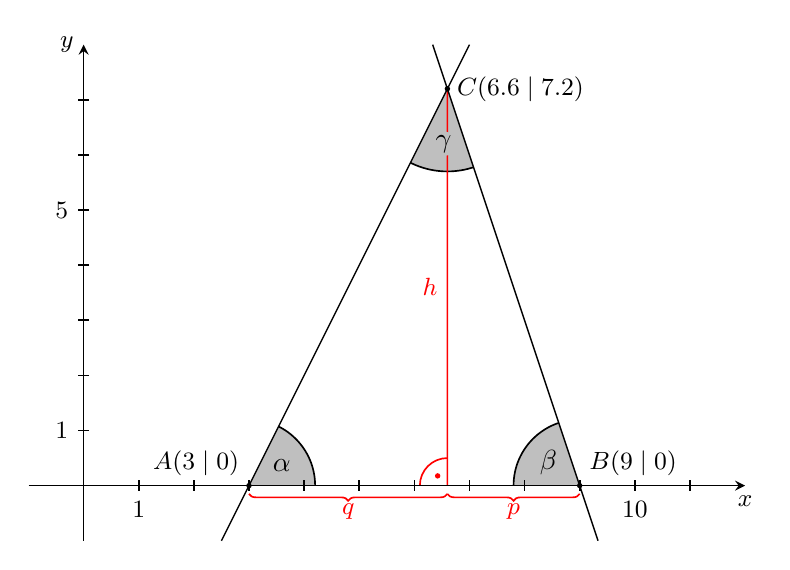
\begin{tikzpicture}[scale=0.7]
    % line coordinates
    \coordinate (A1) at (6.333,   8.000);
    \coordinate (A2) at (9.333,  -1.000);
    \coordinate (B1) at (2.500,  -1.000);
    \coordinate (B2) at (7.000,   8.000);
    % point coordinates
    \coordinate (A) at (3, 0);
    \coordinate (B) at (9, 0);
    \coordinate (C) at (6.6, 7.2);
    % angles
    \begin{scope}
      \clip (A) -- (B) -- (C) -- cycle;
      \fill[fill=black!25!white] (A) circle[radius=12mm];
      \fill[fill=black!25!white] (B) circle[radius=12mm];
      \fill[fill=black!25!white] (C) circle[radius=15mm];
      \draw[line width=0.6pt] (A) circle[radius=12mm];
      \draw[line width=0.6pt] (B) circle[radius=12mm];
      \draw[line width=0.6pt] (C) circle[radius=15mm];
      \node at ([shift={(31.71745:7mm)}]A) {$\alpha$};
      \node at ([shift={(144.21745:7mm)}]B) {$\beta$};
    \end{scope}
    % p, q and h
    \begin{scope}[draw=red]
      \draw[line width=0.6pt] (C) -- node[left]{\small\textcolor{red}{$h$}} (6.6, 0);
      \draw[line width=0.6pt, decorate, decoration=brace, yshift=-1.5mm] (6.6, 0) -- node[below]{\small\textcolor{red}{$q$}} (3, 0);
      \draw[line width=0.6pt, decorate, decoration=brace, yshift=-1.5mm] (9, 0) -- node[below]{\small\textcolor{red}{$p$}} (6.6, 0);
      \clip (0, 0) -- (6.6, 0) -- (C) -- cycle;
      \draw[line width=0.6pt] (6.6, 0) circle[radius=5mm];
      \fill[fill=red, shift={(135:2.5mm)}] (6.6, 0) circle[radius=1.4pt];
    \end{scope}
    % gamma above red lines
    \begin{scope}
      \clip (A) -- (B) -- (C) -- cycle;
      \fill[fill=black!25!white] ([shift={(265.9349:10mm)}]C) circle[radius=2.25mm];
      \node at ([shift={(265.9349:10mm)}]C) {$\gamma$};
    \end{scope}
    % x-axis
    \draw[line width=0.6pt, ->, >=stealth] (-1.000, 0) -- (12.000, 0) node[below] {\small$x$};
    % x scale
    \draw[line width=0.6pt] ( 1, 0.1) -- ( 1, -0.1) node[below] {\small1};
    \draw[line width=0.6pt] ( 2, 0.1) -- ( 2, -0.1);
    \draw[line width=0.6pt] ( 3, 0.1) -- ( 3, -0.1);
    \draw[line width=0.6pt] ( 4, 0.1) -- ( 4, -0.1);
    \draw[line width=0.6pt] ( 5, 0.1) -- ( 5, -0.1);
    \draw[line width=0.6pt] ( 6, 0.1) -- ( 6, -0.1);
    \draw[line width=0.6pt] ( 7, 0.1) -- ( 7, -0.1);
    \draw[line width=0.6pt] ( 8, 0.1) -- ( 8, -0.1);
    \draw[line width=0.6pt] ( 9, 0.1) -- ( 9, -0.1);
    \draw[line width=0.6pt] (10, 0.1) -- (10, -0.1) node[below] {\small10};
    \draw[line width=0.6pt] (11, 0.1) -- (11, -0.1);
    % y-axis
    \draw[line width=0.6pt, ->, >=stealth] (0, -1.000) -- (0, 8.000) node[left] {\small$y$};
    % y scale
    \draw[line width=0.6pt] (0.1, 1) -- (-0.1, 1) node[left] {\small1};
    \draw[line width=0.6pt] (0.1, 2) -- (-0.1, 2);
    \draw[line width=0.6pt] (0.1, 3) -- (-0.1, 3);
    \draw[line width=0.6pt] (0.1, 4) -- (-0.1, 4);
    \draw[line width=0.6pt] (0.1, 5) -- (-0.1, 5) node[left] {\small5};
    \draw[line width=0.6pt] (0.1, 6) -- (-0.1, 6);
    \draw[line width=0.6pt] (0.1, 7) -- (-0.1, 7);
    % lines
    \draw[line width=0.5pt] (A1) -- (A2);
    \draw[line width=0.5pt] (B1) -- (B2);
    % points
    \fill (3, 0) circle[radius=1.4pt] node[above left]{\small$A(3\mid0)$};
    \fill (9, 0) circle[radius=1.4pt] node[above right]{\small$B(9\mid0)$};
    \fill (6.6, 7.2) circle[radius=1.4pt] node[right]{\small$C(\num{6.6}\mid\num{7.2})$};
  \end{tikzpicture}
\end{frame}

\begin{frame}
  \frametitle{\sectiontitle}
  Die Winkel $\alpha$ und $\beta$ erhält man z.\,B. aus der
  Umkehrung der Tangensfunktion:
  \begin{equation*}
    \begin{split}
      \alpha&=\arctan\left(\frac{h}{q}\right)
             =\arctan\left(\frac{\num{7.2}}{\num{3.6}}\right)
             \approx\num{63.43}^\circ \\[2ex]
       \beta&=\arctan\left(\frac{h}{p}\right)
             =\arctan\left(\frac{\num{7.2}}{\num{2.4}}\right)
             \approx\num{71.57}^\circ
    \end{split}
  \end{equation*}
  \medskip

  \pause

  Den fehlenden dritten Winkel kann man leicht mithilfe der Innenwinkelsumme
  von Dreiecken bestimmen:
  \begin{equation*}
    \gamma=180^\circ-\alpha-\beta=45^\circ
  \end{equation*}
\end{frame}

% ------------------------------------------------------------------------------
\end{document}
% ------------------------------------------------------------------------------

